% =============================================================================
% COMP9444 Group Project 047 -- SUBMISSION VERSION of the Summary Report.
%
% HARD CONSTRAINT: the marking criteria allow "max 4 pages, excl. references",
% and the 1-mark "Overall quality" criterion explicitly requires being within
% that length. This file is therefore laid out two-column at 10pt and MUST end
% its Conclusions on page 4; the bibliography spills onto page 5, which is
% excluded from the count.
%
% The long-form master document is report_sections.tex (~27 pages). Every number
% here is copied from it and is ultimately traceable to Models/results/*.json.
% If you edit a number, edit it there first.
% =============================================================================
\documentclass[10pt,twocolumn]{article}

\usepackage[utf8]{inputenc}
\usepackage[T1]{fontenc}
\usepackage[margin=0.68in]{geometry}
\setlength{\columnsep}{0.24in}
\usepackage{amsmath,amssymb}
\usepackage{graphicx}
\usepackage{booktabs}
\usepackage{tabularx}
\usepackage{caption}
\usepackage{xcolor}
\usepackage{float}
\usepackage{cite}
\usepackage[hidelinks]{hyperref}
\graphicspath{{figures/}{Models/results/figures/}{EDA/figures/}}

\captionsetup{font=small,labelfont=bf,skip=3pt}
\setlength{\abovecaptionskip}{3pt}
\setlength{\belowcaptionskip}{2pt}
\setlength{\textfloatsep}{6pt}
\setlength{\floatsep}{6pt}
\setlength{\intextsep}{6pt}
\setlength{\parskip}{0pt}
\emergencystretch=3em

\newcommand{\best}[1]{\textbf{#1}}
\newcolumntype{Y}{>{\raggedright\arraybackslash}X}

% tighter section headings
\usepackage{titlesec}
\titlespacing*{\section}{0pt}{5pt}{2pt}
\titlespacing*{\subsection}{0pt}{4pt}{1pt}
\titleformat{\section}{\normalfont\large\bfseries}{\thesection}{0.6em}{}
\titleformat{\subsection}{\normalfont\normalsize\bfseries}{\thesubsection}{0.6em}{}

\title{\vspace{-2.4em}\textbf{Breast Cancer Classification and Segmentation on
Ultrasound Images:\\ A Leakage-Free Benchmark, an Improved Segmenter, and a
Rigorously Evaluated Classifier}\vspace{-0.5em}}
% TODO(team): replace the placeholders below with each member's zID and full name,
% exactly as the .docx template asks ("Write your zIDs and names here").
\author{\normalsize COMP9444 Group \emph{AreuOk?} --- Project 047\\[2pt]
\normalsize z0000000 Name One \quad z0000000 Name Two \quad z0000000 Name Three\\
\normalsize z0000000 Name Four \quad z0000000 Name Five\vspace{-1.2em}}
\date{}

\begin{document}
\maketitle

\begin{abstract}
\noindent\small
Breast ultrasound (BUS) is safe and cheap but hard to interpret, and its main
public benchmark, BUSI, is small, imbalanced and full of near-duplicate images.
We study lesion segmentation and image classification on BUSI under one cleaned,
\emph{leakage-free} protocol. Perceptual hashing shows that $36\%$ of BUSI lies in
near-duplicate clusters and that an exact cross-class duplicate exists, so we
split at the cluster level. Under this protocol we reproduce thirteen published
models and add two of our own. A controlled ablation shows an ImageNet-pretrained
encoder alone raises Dice from $0.648$ to $0.765$ and accounts for essentially all
of our segmenter's gain, while a Focal-Tversky loss, test-time augmentation and
attention gates do not improve overlap. A controlled Stage-1 substitution shows
the dual-stage pipeline is limited by its \emph{classifier}, not its segmenter.
Evaluated rigorously (out-of-fold training masks, five seeds, bootstrap $95\%$
CIs), hand-crafted shape/radiomics features give no reliable gain and only
ensembling survives, reaching macro-F1 $0.875$ ($95\%$ CI $[0.80,0.94]$). Our
reproductions fall below their published numbers, which we attribute to removing
leakage. This is a decision-support study, not autonomous diagnosis.

\vspace{4pt}
\noindent\textit{\textbf{Keywords}}---breast ultrasound; BUSI; medical image
segmentation; image classification; U-Net; transfer learning; data leakage;
near-duplicate detection; ablation study; bootstrap confidence interval;
computer-aided diagnosis.
\end{abstract}

% =============================================================================
\section{Introduction}
% =============================================================================
Breast cancer is a leading cause of cancer death in women and early detection is
the most effective way to reduce mortality~\cite{cheng2010survey}. Breast
ultrasound is safe, cheap and radiation-free, and works well on dense tissue where
mammography loses sensitivity, but it is hard to read: speckle noise, low
contrast, acoustic shadowing and blurred boundaries make manual assessment slow
and operator-dependent~\cite{xian2018survey}. \emph{Classification} answers
\emph{what} a scan shows (normal / benign / malignant); \emph{segmentation}
answers \emph{where} the lesion is, supporting interpretability, measurement, and
a classifier focused on the lesion rather than surrounding clutter. Automating
both would let a computer-aided diagnosis system triage screening studies and give
the radiologist a second reading, which is the practical application we target.

Following the Project~047 brief we build and evaluate a system on the BUSI
dataset~\cite{aldhabyani2020busi} for both tasks. Our central concern is
\emph{trustworthy comparison}: BUSI is small, imbalanced and, as we show, riddled
with near-duplicates, so a careless split inflates scores substantially. We
therefore build one cleaned, leakage-free protocol and put every model through it.
Four questions organise the work. \textbf{RQ1:} how do established architectures
perform under it, versus their published numbers? \textbf{RQ2:} which design
decisions actually matter on data this small? \textbf{RQ3:} does better
segmentation improve downstream classification? \textbf{RQ4:} are apparent gains
stable across seeds and resampling?

\textbf{Contributions.} (i)~A near-duplicate analysis of BUSI and a
cluster-grouped, class-stratified leakage-free split. (ii)~A unified reproduction
of \emph{thirteen} published models -- eight segmenters, three classification
backbones, one dual-stage pipeline, one multi-task network -- under that single
protocol. (iii)~An improved pretrained-encoder segmenter with a controlled
ablation isolating each ingredient. (iv)~An improved dual-stage classifier with a
controlled Stage-1 substitution and a ground-truth-ROI upper-bound diagnostic.
(v)~A rigorous evaluation protocol (out-of-fold masks, multi-seed ensembling,
bootstrap CIs) that separates real improvements from noise.

% =============================================================================
\section{Related Work}
% =============================================================================
Classical BUS CAD chained pre-processing, segmentation, feature extraction and
classification; the surveys of Cheng et al.~\cite{cheng2010survey} and Xian et
al.~\cite{xian2018survey} recur to the same obstacles that persist today. BUSI
\cite{aldhabyani2020busi} is the de-facto benchmark because it supplies both labels
and pixel masks. A documented data-quality issue -- repeated and near-duplicate
frames, some with conflicting labels -- has been raised for it~\cite{pawlowska2023};
we quantify this directly and design our evaluation around it.

\textbf{Classification.} ResNet~\cite{he2016resnet} made very deep networks
trainable via identity shortcuts; DenseNet~\cite{huang2017densenet} promotes
feature reuse, attractive on small data; EfficientNet~\cite{tan2019efficientnet}
compound-scales depth/width/resolution and transfers well to medical images in its
small variants. Applied to BUSI, Latha et al.~\cite{latha2024effnetb7} report
$\approx99\%$ accuracy with EfficientNet-B7; such near-perfect numbers on so small
a dataset invite suspicion of leakage, which directly motivates our protocol.

\textbf{Segmentation.} U-Net~\cite{ronneberger2015unet} is the foundational
encoder--decoder with skips and trains well from few images; UNet++
\cite{zhou2018unetpp} adds nested skips. Yap et al.~\cite{yap2018cnn} first applied
deep learning to BUS lesion detection, comparing a patch LeNet, a U-Net and a
transfer-learned FCN-AlexNet (best). Attention U-Net~\cite{oktay2018attentionunet}
gates the skips so the network learns where to look;
DeepLabV3+~\cite{chen2018deeplabv3plus} adds atrous separable convolutions and ASPP
for multi-scale context; nnU-Net~\cite{isensee2021nnunet} self-configures the whole
pipeline and remains a strong general baseline. Two designs target BUS
specifically: AAU-Net~\cite{chen2023aaunet} replaces convolutions with a hybrid
adaptive attention module for blurred boundaries, and
CResU-Net~\cite{derakhshandeh2024cresunet} schedules specialised residual/dense
blocks and reports the strongest BUSI Dice in this literature. Foundation
segmenters (SAM~\cite{kirillov2023sam}, MedSAM~\cite{ma2024medsam}) need prompts or
adaptation, so we treat them as context, not baselines. For the combined task,
Bruno et al.~\cite{bruno2025dualstage} propose a \emph{sequential} pipeline
(segment, crop the ROI, classify it) whereas Lu et al.~\cite{lu2025multitask} use
\emph{joint} multi-task learning with a shared encoder; these two lines frame our
design space.

\textbf{Limitations of existing work.} Three recur. Reported BUSI scores use
different splits and pre-processing, so they are not comparable across papers;
most studies report a \emph{single} run with no seeds or confidence intervals, on
a test set far too small to resolve the differences they claim; and none
de-duplicates, so near-duplicates leak across a naive split and inflate every
number. Our protocol addresses each in turn, which is what makes the reproductions
below comparable to one another even though they are lower than published values.

% =============================================================================
\section{Methods}
% =============================================================================
\subsection{Reproduced models}
All models share the same split, letterbox pre-processing, augmentation and metric
code from \texttt{Models/common/}, so differences reflect architecture and recipe,
not data handling. For every model we wrote the head/decoder and the
training/evaluation loop ourselves; pretrained backbones are torchvision or
\texttt{segmentation-models-pytorch} components. We reproduce the brief's three
required papers -- a from-scratch \textbf{U-Net}~\cite{ronneberger2015unet}, Yap's
\textbf{patch LeNet} and \textbf{FCN-AlexNet}~\cite{yap2018cnn} -- plus
\textbf{Attention U-Net}~\cite{oktay2018attentionunet} (identical recipe to our
U-Net, hence a controlled test of the attention gate),
\textbf{DeepLabV3+}~\cite{chen2018deeplabv3plus} (pretrained ResNet-50 + ASPP),
\textbf{nnU-Net}~\cite{isensee2021nnunet} (blueprint 2D U-Net, deep supervision),
\textbf{AAU-Net}~\cite{chen2023aaunet} (HAAM module from scratch) and
\textbf{CResU-Net}~\cite{derakhshandeh2024cresunet} (pure Dice loss as published).
For classification we fine-tune the \emph{smallest} variant of each family --
\textbf{ResNet-18}, \textbf{DenseNet-121}, \textbf{EfficientNet-B0} -- with a fresh
three-way head and weighted cross-entropy, because BUSI is small. For the combined
task we reproduce Bruno's \textbf{dual-stage} pipeline and Lu's \textbf{MTL-OCA}
multi-task network.

\subsection{Our two proposed models}
\label{sec:proposed}
\textbf{Improved segmenter.} The only reproduced segmenter using transfer learning
(DeepLabV3+) clearly out-scored the from-scratch ones, so we hypothesise that
\emph{transfer learning is the decisive factor} on BUSI. We therefore build a
U-Net whose encoder is an ImageNet-pretrained \textbf{EfficientNet-B4}, keeping the
U-Net decoder and skips ($20.2$\,M parameters). On top we test two EDA-driven
ideas: a \textbf{Focal-Tversky\,+\,BCE} loss and \textbf{TTA + post-processing}.
The Tversky index $T=\mathrm{TP}/(\mathrm{TP}+\alpha\,\mathrm{FP}+\beta\,\mathrm{FN})$
weights false positives and negatives asymmetrically (soft counts, per image), and
the focal variant is $\mathcal{L}_{\mathrm{FT}}=(1-T)^{\gamma}$
\cite{abraham2019focaltversky}. We train with
$\mathcal{L}=\lambda\mathcal{L}_{\mathrm{BCE}}+(1-\lambda)\mathcal{L}_{\mathrm{FT}}$,
$\lambda=0.5$, $(\alpha,\beta,\gamma)=(0.3,0.7,\tfrac43)$ -- the published
defaults, \emph{not} tuned on our data, so the ablation stays honest; since
$\alpha{=}\beta{=}0.5,\gamma{=}1$ recovers Dice exactly, this strictly generalises
the baseline loss. At inference TTA averages the probability maps of the image,
its horizontal flip and two rescalings; the result is thresholded at $0.5$, closed
with a $5\times5$ ellipse and reduced to its largest connected component.

\textbf{Improved dual-stage pipeline.} We make three changes to Bruno's pipeline
and evaluate them rigorously. \emph{(i)~Stronger Stage-1:} we substitute our
segmenter and keep the ROI coupling and Stage-2 classifier byte-for-byte identical,
so any change is attributable to segmentation alone. The coupling is fixed
throughout: largest 8-connected component, bounding box dilated by $15\%$ per side,
rejected below $16$\,px, falling back to the whole frame if the mask is empty,
resized to $256\times256$. \emph{(ii)~Strengthened Stage-2:} the original trains on
clean ground-truth ROI crops but tests on imperfect predicted crops -- a
distribution mismatch. We train on \emph{both}, select on predicted-ROI validation
macro-F1, and add flip TTA. \emph{(iii)~Feature fusion:} we optionally concatenate
$6$ shape descriptors (area ratio, circularity, solidity, extent, bbox aspect,
eccentricity) or a $14$-D radiomics vector ($+3$ intensity, $+5$ GLCM texture) to
the pooled CNN embedding, always computed from the \emph{predicted} mask so the
classifier never sees geometry it would lack at deployment.

% =============================================================================
\section{Experiments}
% =============================================================================
\textbf{Dataset.} We use the Breast Ultrasound Images (BUSI)
dataset~\cite{aldhabyani2020busi}, collected in 2018 at Baheya Hospital, Cairo,
from $600$ female patients aged $25$--$75$. It holds $780$ grayscale PNG scans
(average $\approx500\times500$\,px), each with a label in \{normal, benign,
malignant\} and one or more pixel-level lesion masks; normal scans carry an empty
mask. Source:
\href{https://huggingface.co/datasets/gymprathap/Breast-Cancer-Ultrasound-Images-Dataset}%
{\texttt{huggingface.co/datasets/\allowbreak gymprathap/Breast-Cancer-\allowbreak
Ultrasound-Images-Dataset}}.

\textbf{Key EDA findings.} The classes are imbalanced -- benign $437$ ($56\%$),
malignant $210$ ($27\%$), normal $133$ ($17\%$) -- so we report
\emph{macro}-averaged metrics rather than accuracy and weight the loss by inverse
class frequency. Sizes vary ($639$ distinct resolutions), so we resize \emph{with
padding} to $256\times256$ to preserve the discriminative lesion aspect ratio.
Malignant lesions occupy a far larger area ratio (median $\approx12\%$ vs.\
$\approx4\%$) and many benign lesions are tiny, creating a severe pixel-level
foreground imbalance that favours an overlap-aware loss; they are also less
circular and solid and more eccentric, motivating both attention-based segmenters
and the shape-feature fusion of Section~\ref{sec:proposed}. Lesions concentrate
near the image centre, so we augment with small translations.

\textbf{The decisive finding} is a data-integrity one. MD5 hashing reveals an
\emph{exact cross-class duplicate}: \texttt{benign(433).png} and
\texttt{malignant(145).png} are byte-identical but carry different labels.
Perceptual hashing (Hamming $\leq5$) finds $186$ near-duplicate pairs, $10$ of them
crossing class boundaries, forming $124$ clusters that cover $277$ images -- $36\%$
of BUSI. Simulating naive random $70/30$ splits, on the order of $57$ clusters end
up with copies on \emph{both} sides, so the test set contains images the model
effectively trained on. Our remedy: drop the conflicting duplicate, union-merge
multi-mask images, and split at the \emph{cluster} level while stratifying by class.

\textbf{Split.} One cluster-grouped, class-stratified split is built once and
cached, so every training script reads the same file: clusters (not images) are
shuffled with seed $42$ within each class and allocated $70/15/15$. Segmentation
uses the $645$ lesion images, split $445/102/98$ over $532$ clusters;
classification uses all $778$ retained images, split $540/120/118$ over $626$
clusters; the dual-stage pipeline is scored on the $98$-image two-class test
subset. A programmatic check confirms \textbf{zero} clusters span more than one
split -- the assertion that makes the benchmark leakage-free. Augmentation
(horizontal flip $p{=}0.5$; affine scale $[0.9,1.1]$, translation $\pm5\%$,
rotation $\pm15^\circ$; brightness/contrast $\pm0.2$, $p{=}0.3$) is applied to the
training split only. We deliberately omit vertical flips: an ultrasound frame has a
fixed top-down geometry.

\textbf{Training.} Each model follows its source paper's recipe where practical,
rather than a single forced recipe that would misrepresent the reproductions; all
inputs are $256\times256$. Segmenters use Adam/AdamW at $10^{-3}$--$10^{-4}$ for
$60$--$120$ epochs (batch $8$), except nnU-Net ($200$ epochs, SGD-Nesterov $0.99$,
poly$^{0.9}$) and MTL-OCA ($300$). Classifiers use batch $16$, $20$--$60$ epochs,
weighted cross-entropy. Our improved segmenter uses AdamW ($10^{-3}$, cosine, $60$
epochs), the improved Stage-2 Adam ($10^{-4}$, cosine, $60$). Masks are
thresholded at a fixed $0.5$; Patch-LeNet's detection threshold was tuned on
validation only ($0.8$). All selection uses train/validation only.

\textbf{Metrics.} Segmentation: per-image Dice and IoU (primary, averaged over
images so large lesions do not dominate), pixel precision/recall and Yap's
detection metrics (true-positive fraction, FP per image, F-measure).
Classification: macro-F1 (primary), balanced accuracy, accuracy, per-class
P/R/F1 and macro one-vs-rest AUC. Macro-F1 is preferred because accuracy can look
high while the minority malignant class is handled badly.

\textbf{Statistical protocol.} For the final pipeline we go beyond single runs.
Each configuration is trained with \emph{five seeds}; we report the per-seed
mean$\pm$std and a five-model probability-averaged \emph{ensemble}, plus a
percentile \emph{bootstrap} $95\%$ CI ($B=2000$ resamples of the $98$ test images)
for test-set uncertainty. Predicted \emph{training} masks are generated
\emph{out-of-fold} by five-fold cross-fitting, so each training image's mask comes
from a segmenter that never saw it -- a correctness measure, not a way to raise the
score. Overlapping CIs are treated as evidence that a difference is \emph{not}
resolved. Everything ran on one RTX~5060 laptop GPU (PyTorch $2.10$, CUDA $12.8$),
so wall-clock times are comparable; total compute is about six GPU-hours.

% =============================================================================
\section{Results}
% =============================================================================
\subsection{Segmentation}
Our improved segmenter is best (Dice $\best{0.760}$, IoU $0.688$), ahead of
DeepLabV3+ ($0.739$) and both BUS-specific SOTA reproductions
(Table~\ref{tab:seg}). Three findings follow. First, our reproductions score
\emph{below} their published numbers (AAU-Net $0.730$ vs.\ $0.775$; CResU-Net
$0.693$ vs.\ $0.829$), consistent with removing the near-duplicate leakage the
original protocols did not. Second, nnU-Net ($0.717$), the general ``strong
baseline'', does \emph{not} dominate here -- the transfer-learning models beat it.
Third, the controlled pair Attention U-Net ($0.629$) vs.\ U-Net ($0.648$), which
share an identical recipe, shows the attention gate does not help on this data.
Almost every model is precision-dominant, so the shared failure mode is
under-segmentation; ours is the only one whose recall exceeds its precision, the
clinically preferable direction and the intended effect of the FN-weighted loss.

\begin{table}[t]
\centering
\caption{Segmentation on the leakage-free test set ($98$ images), by Dice.
$\sigma$ = per-image Dice std; P/R = pixel precision/recall; F$_{\mathrm{det}}$ =
Yap detection F-measure; ``Paper'' = published BUSI Dice where available.}
\label{tab:seg}
\scriptsize
\setlength{\tabcolsep}{2.3pt}
\resizebox{\columnwidth}{!}{%
\begin{tabular}{@{}lcccccccc@{}}
\toprule
Model & Dice & $\sigma$ & IoU & P & R & F$_{\mathrm{det}}$ & M & Paper \\
\midrule
\best{Improved U-Net (ours)} & \best{.760} & .307 & \best{.688} & .765 & .790 & \best{.854} & 20.2 & -- \\
DeepLabV3+~\cite{chen2018deeplabv3plus}   & .739 & .290 & .652 & .765 & .753 & .810 & 26.7 & -- \\
AAU-Net~\cite{chen2023aaunet}             & .730 & \best{.284} & .638 & .739 & .759 & .723 & 42.7 & .775 \\
nnU-Net~\cite{isensee2021nnunet}          & .717 & .299 & .627 & .754 & .719 & .781 & 8.5 & -- \\
CResU-Net~\cite{derakhshandeh2024cresunet}& .693 & .305 & .600 & .759 & .697 & .772 & 33.5 & .829 \\
U-Net~\cite{ronneberger2015unet}          & .648 & .362 & .570 & \best{.775} & .637 & .779 & 31.0 & -- \\
Attn.\ U-Net~\cite{oktay2018attentionunet}& .629 & .345 & .540 & .701 & .638 & .631 & 31.4 & -- \\
MTL-OCA~\cite{lu2025multitask} (seg)      & .612 & .332 & .515 & .737 & .598 & .539 & 8.2 & -- \\
FCN-AlexNet~\cite{yap2018cnn}             & .582 & .310 & .471 & .648 & .647 & .804 & 28.7 & -- \\
Patch-LeNet~\cite{yap2018cnn}             & .285 & .268 & .198 & .641 & .223 & .598 & 0.4 & -- \\
\bottomrule
\end{tabular}}
\end{table}

\textbf{Ablation (Table~\ref{tab:abl}).} The result is unambiguous: the pretrained
encoder is responsible for essentially the \emph{entire} gain, raising Dice from
$0.648$ to $0.765$ ($+0.117$) and cutting the Dice std from $0.362$ to $0.285$ --
i.e.\ far fewer completely-missed lesions. It is also the \emph{cheapest} model to
train ($7.9$ vs.\ $58.5$ min for the U-Net it replaces), because pretraining
converges in far fewer epochs. Focal-Tversky does \emph{not} raise Dice
($-0.005$); consistent with its design it trades $2.4$ points of precision for
$3.7$ of recall and recovers two more lesions. Dice, symmetric in FP and FN, is
almost blind to that reallocation -- which is why we report the breakdown rather
than resting on the headline. TTA leaves Dice unchanged but cuts false positives by
a quarter. We therefore explicitly \emph{do not} claim Focal-Tversky or TTA improve
overlap; their effects are on recall and output cleanliness.

\begin{table}[t]
\centering
\caption{Controlled ablation of the improved segmenter. Each row adds one
component; split, pre-processing, augmentation and schedule are held fixed.}
\label{tab:abl}
\scriptsize
\setlength{\tabcolsep}{2.3pt}
\resizebox{\columnwidth}{!}{%
\begin{tabular}{@{}lcccccc@{}}
\toprule
Configuration & Dice & $\Delta$ & $\sigma$ & Pix.\,P & Pix.\,R & FP/img \\
\midrule
From-scratch U-Net (Dice+BCE) & .648 & --- & .362 & .775 & .637 & .296 \\
$+$ pretrained EffB4 enc. & \best{.765} & $+.117$ & .285 & \best{.799} & .763 & .214 \\
$+$ Focal-Tversky loss & .760 & $-.005$ & \best{.282} & .775 & \best{.800} & .225 \\
$+$ TTA $+$ post-proc.\ (full) & .760 & $\pm.000$ & .307 & .765 & .790 & \best{.163} \\
\bottomrule
\end{tabular}}
\end{table}

\subsection{Classification}
EfficientNet-B0 is best (macro-F1 $\best{0.828}$, balanced accuracy $0.852$, AUC
$0.969$), ahead of ResNet-18 ($0.810$) and DenseNet-121 ($0.793$); all three
pretrained backbones clearly beat MTL-OCA ($0.720$). Per-class F1 for the best
model is normal $0.766$, benign $0.884$, malignant $0.833$, with malignant recall
$0.807$ -- this per-class view, not the overall accuracy of $0.848$, is the
operative summary for an imbalanced clinical task. The ranking also hides a
clinically relevant detail: ResNet-18 is \emph{more sensitive} on malignant
($R=0.839$, one more of $31$ caught) though less precise, so it is arguably the
better operating point despite ranking second. MTL-OCA underperforms on \emph{both}
tasks (Dice $0.612$, macro-F1 $0.720$): sharing one backbone across tasks is, on
data this small, worse than a specialised network per task.

\subsection{Dual-stage pipeline}
\textbf{Controlled Stage-1 substitution (RQ3).} Substituting our stronger
segmenter raises Stage-1 Dice from $0.739$ to $0.760$ but moves single-run
end-to-end macro-F1 only from $0.804$ to $0.807$ -- about $0.14$ points of F1 per
point of Dice. The GT-ROI diagnostic explains why: feeding the \emph{same}
classifier perfect crops reaches only $0.865$--$0.884$, so the score recoverable by
perfect segmentation is $0.06$--$0.08$ and does not shrink as Stage-1 improves.
Concretely, the pipeline misclassifies $16$ of $98$ images and the oracle
misclassifies $10$: perfect masks repair six errors and leave ten standing. A mask
with Dice $0.76$ already crops a useful ROI, so the system is
\emph{classifier-bound}, not segmentation-bound.

\textbf{Rigorous evaluation (RQ4).} The single-run ladder looks like a tidy climb
($0.804\!\to\!0.840$), but under out-of-fold masks, five-seed ensembling and
bootstrap CIs the variants' intervals overlap almost entirely
(Table~\ref{tab:dual}, Fig.~\ref{fig:ci}). Re-running the \emph{identical}
configuration with only the seed changed moves macro-F1 by up to $0.039$ --
comparable to the entire $0.036$ ``improvement'' of the ladder; a study reporting
the shape variant's luckiest seed against a no-feature unlucky one would ``show''
a $+0.043$ gain that is pure noise. Hand-crafted features give \emph{no reliable}
gain: \emph{none} and \emph{shape} both ensemble to $0.875$. Only
\emph{ensembling} survives (per-seed $0.847\to$ ensemble $0.875$, above even the
best individual seed). Our best defensible result is macro-F1 $\best{0.875}$
($95\%$ CI $[0.80,0.94]$), malignant recall $0.903$.

\begin{table}[t]
\centering
\caption{Improved dual-stage pipeline, two-class $98$-image test set, evaluated
with out-of-fold training masks, five seeds and a bootstrap $95\%$ CI ($B=2000$).
All three intervals overlap; only ensembling reliably helps.}
\label{tab:dual}
\scriptsize
\setlength{\tabcolsep}{3.4pt}
\begin{tabular}{@{}lcccc@{}}
\toprule
Configuration & Ens.\ F1 & Per-seed & $95\%$ CI & Malig.\,R \\
\midrule
OOF, no hand features & \best{.875} & $.847\!\pm\!.011$ & $[.800,.936]$ & \best{.903} \\
OOF $+$ shape ($6$)   & \best{.875} & $.861\!\pm\!.016$ & $[.800,.936]$ & \best{.903} \\
OOF $+$ radiomics ($14$) & .863 & $.862\!\pm\!.013$ & $[.785,.929]$ & .871 \\
\bottomrule
\end{tabular}
\end{table}

\begin{figure}[t]
\centering
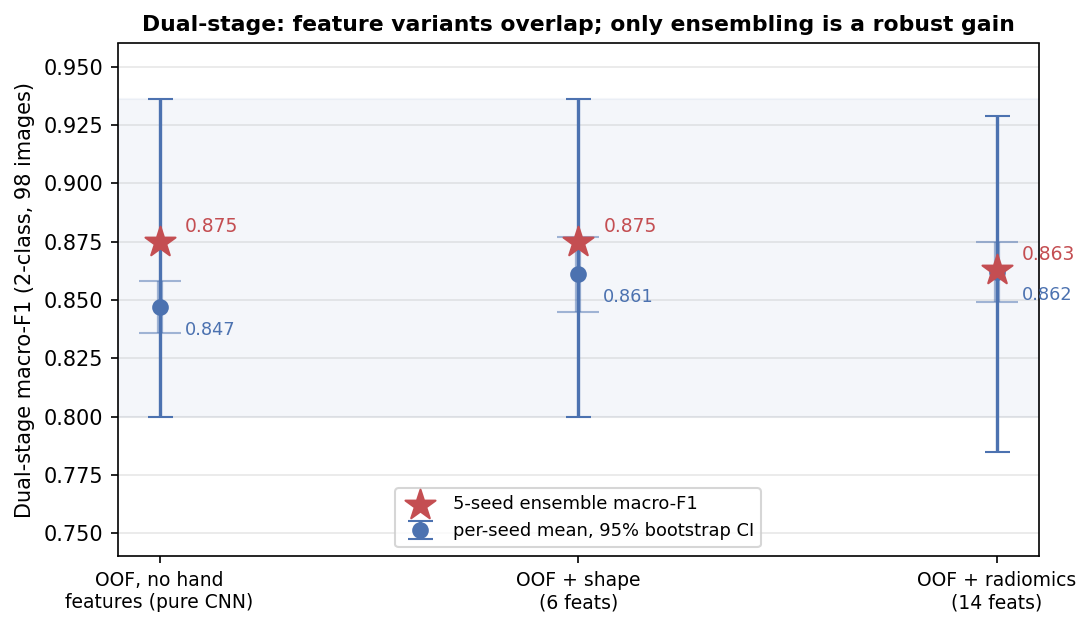
\includegraphics[width=0.66\linewidth]{fig_dualstage_ci}
\caption{The three feature variants' bootstrap $95\%$ CIs overlap almost
entirely; only ensembling (stars) reliably lifts the per-seed mean (dots).}
\label{fig:ci}
\end{figure}

\subsection{Error analysis}
Classification confusion concentrates on the malignant class and the
benign$\leftrightarrow$malignant boundary, matching the EDA finding that the two
overlap in intensity. Segmentation errors track lesion difficulty -- small
low-contrast lesions and irregular malignant boundaries drive the large Dice std,
and the worst cases are near-complete \emph{misses} rather than uniform boundary
error, exactly the sub-population the pretrained encoder most improves. In the
pipeline the residual errors are classification errors on correctly localised
lesions.

% =============================================================================
\section{Conclusion}
% =============================================================================
\textbf{Answers.} \emph{RQ1:} transfer-learned models lead each task and reproduced
SOTA scores below published values. \emph{RQ2:} the pretrained encoder is decisive
($+0.117$ Dice); loss, attention, TTA and nnU-Net add little. \emph{RQ3:} better
segmentation does \emph{not} improve the pipeline -- it is classifier-bound.
\emph{RQ4:} single-run gains are unstable; only ensembling survives.

\textbf{Strengths.} The dominant factor shaping our numbers is evaluation hygiene,
and that discipline -- remove leakage, attribute gains with controlled ablations,
report multi-seed results with CIs -- is the project's central contribution. That
published scores fall sharply under a cluster-grouped split does not mean our
implementations are weak; it means BUSI leaderboard numbers are incomparable unless
splitting and de-duplication match. Measuring the bottleneck with a ground-truth
upper bound \emph{before} investing in the more visible component is a transferable
lesson.

\textbf{Limitations.} (i)~All results come from one small dataset and one split;
$98$ test images cannot resolve small differences, and the test-set uncertainty
($\pm0.07$) dwarfs the training uncertainty ($\pm0.01$), so no number of seeds
would fix this. (ii)~No external or multi-centre validation. (iii)~BUSI itself has
near-duplicate and annotation issues. (iv)~We use static 2D frames and the data
carry acquisition bias. (v)~Compute limited our search: we ran no CLAHE/denoising
ablation, a deliberate omission rather than evidence those steps are useless.
(vi)~Our reproductions may differ in detail from the original code, and the
dual-stage task is two-class, so not comparable to the three-class classifiers. We
therefore interpret the system as \emph{decision support}: none of these numbers
would justify unsupervised clinical use. \textbf{Given more time} we would add
external multi-centre and nested cross-validation; audit the classifiers with
Grad-CAM to confirm they attend to the lesion, not to burned-in annotations; and,
since the pipeline is classifier-bound, invest in stronger ROI classifiers and
self-supervised pretraining rather than in the segmenter.

% =============================================================================
\begingroup
\footnotesize
\begin{thebibliography}{99}
\itemsep0pt
% =============================================================================
\bibitem{aldhabyani2020busi}
W.~Al-Dhabyani, M.~Gomaa, H.~Khaled, and A.~Fahmy, ``Dataset of breast ultrasound
images,'' \emph{Data in Brief}, vol.~28, 104863, 2020.

\bibitem{yap2018cnn}
M.~H.~Yap et al., ``Automated breast ultrasound lesions detection using
convolutional neural networks,'' \emph{IEEE JBHI}, vol.~22, no.~4, pp.~1218--1226,
2018.

\bibitem{ronneberger2015unet}
O.~Ronneberger, P.~Fischer, and T.~Brox, ``U-Net: Convolutional networks for
biomedical image segmentation,'' in \emph{MICCAI}, pp.~234--241, 2015.

\bibitem{he2016resnet}
K.~He, X.~Zhang, S.~Ren, and J.~Sun, ``Deep residual learning for image
recognition,'' in \emph{CVPR}, pp.~770--778, 2016.

\bibitem{huang2017densenet}
G.~Huang, Z.~Liu, L.~van der Maaten, and K.~Q.~Weinberger, ``Densely connected
convolutional networks,'' in \emph{CVPR}, pp.~4700--4708, 2017.

\bibitem{tan2019efficientnet}
M.~Tan and Q.~V.~Le, ``EfficientNet: Rethinking model scaling for convolutional
neural networks,'' in \emph{ICML}, pp.~6105--6114, 2019.

\bibitem{chen2018deeplabv3plus}
L.-C.~Chen, Y.~Zhu, G.~Papandreou, F.~Schroff, and H.~Adam, ``Encoder-decoder with
atrous separable convolution for semantic image segmentation,'' in \emph{ECCV},
pp.~801--818, 2018.

\bibitem{zhou2018unetpp}
Z.~Zhou, M.~M.~R.~Siddiquee, N.~Tajbakhsh, and J.~Liang, ``UNet++: A nested U-Net
architecture for medical image segmentation,'' in \emph{DLMIA/MICCAI}, pp.~3--11,
2018.

\bibitem{oktay2018attentionunet}
O.~Oktay et al., ``Attention U-Net: Learning where to look for the pancreas,''
\emph{arXiv:1804.03999}, 2018.

\bibitem{chen2023aaunet}
G.~Chen, L.~Li, Y.~Dai, J.~Zhang, and M.~H.~Yap, ``AAU-Net: An adaptive attention
U-Net for breast lesions segmentation in ultrasound images,'' \emph{IEEE TMI},
vol.~42, no.~5, pp.~1289--1300, 2023.

\bibitem{derakhshandeh2024cresunet}
M.~Derakhshandeh and A.~Mahloojifar, ``Modifying the U-Net's encoder-decoder
architecture for segmentation of tumors in breast ultrasound images,''
\emph{J.\ Digital Imaging}, 2024.

\bibitem{latha2024effnetb7}
M.~Latha et al., ``Revolutionizing breast ultrasound diagnostics with
EfficientNet-B7 and Explainable AI,'' \emph{BMC Medical Imaging}, vol.~24, 230,
2024.

\bibitem{bruno2025dualstage}
A.~Bruno et al., ``A dual-stage deep learning framework for breast ultrasound
image segmentation and classification,'' \emph{J.\ Medical Systems}, 2025.

\bibitem{lu2025multitask}
Y.~Lu et al., ``Automatic joint segmentation and classification of breast
ultrasound images via multi-task learning with object contextual attention,''
\emph{Frontiers in Oncology}, vol.~15, 1567577, 2025.

\bibitem{isensee2021nnunet}
F.~Isensee, P.~F.~Jaeger, S.~A.~A.~Kohl, J.~Petersen, and K.~H.~Maier-Hein,
``nnU-Net: A self-configuring method for deep learning-based biomedical image
segmentation,'' \emph{Nature Methods}, vol.~18, pp.~203--211, 2021.

\bibitem{kirillov2023sam}
A.~Kirillov et al., ``Segment Anything,'' in \emph{ICCV}, pp.~4015--4026, 2023.

\bibitem{ma2024medsam}
J.~Ma et al., ``Segment Anything in medical images,'' \emph{Nature
Communications}, vol.~15, 654, 2024.

\bibitem{xian2018survey}
M.~Xian et al., ``Automatic breast ultrasound image segmentation: A survey,''
\emph{Pattern Recognition}, vol.~79, pp.~340--355, 2018.

\bibitem{cheng2010survey}
H.~D.~Cheng et al., ``Automated breast cancer detection and classification using
ultrasound images: A survey,'' \emph{Pattern Recognition}, vol.~43, no.~1,
pp.~299--317, 2010.

\bibitem{abraham2019focaltversky}
N.~Abraham and N.~M.~Khan, ``A novel focal Tversky loss function with improved
attention U-Net for lesion segmentation,'' in \emph{IEEE ISBI}, pp.~683--687,
2019.

\bibitem{pawlowska2023}
A.~Paw{\l}owska, P.~Karwat, and N.~{\.Z}o{\l}ek, ``Letter to the Editor.\ Re:
`Dataset of breast ultrasound images','' \emph{Data in Brief}, vol.~48, 109247,
2023.

\end{thebibliography}
\endgroup

\end{document}
